\section{Reconstruction}
\label{sec:Reconstruction}
The reconstruction process is illustrated in figure~\ref{fig:DataFlow} for both real and simulated data.

\begin{figure}[tbh]
  \begin{center}
    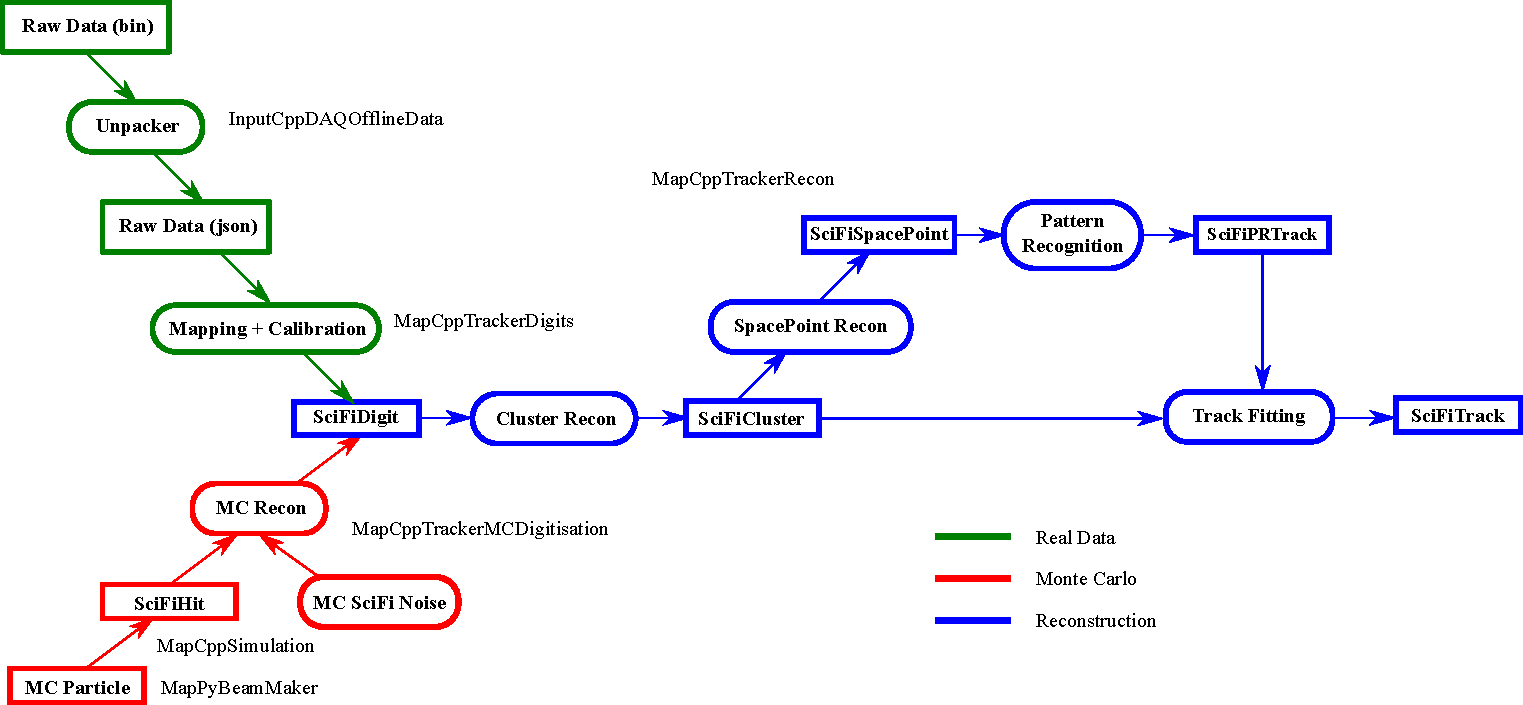
\includegraphics[width=0.95\linewidth]{07-Reconstruction/DataFlow2014.pdf}
    \caption{\label{fig:DataFlow} The reconstruction data flow. Data originates either from simulated or real data, the two branches meet after digitisation, after which the reconstruction proceeds identically for both.  The relevant MAUS modules for each step are indicated.}
  \end{center}
\end{figure}

  \subsection{Digitization}
  \label{subsec:Digitization}
  For real data the electronic signals produced by the VLPCs are digitised using analogue-to-digital converters (ADCs). The DAQ system records the pulse height for each DAQ channel.  Channel-by-channel cailbration constants are used to convert the ADC value to a signal in units of photo-electrons (PE) and the VLPC channel number to tracker channel number.  This information is then used to form a Digit.  The analagous process for Monte Carlo data is described in section~\ref{sec:Simulation}.

  \subsection{Clustering}
  \label{subsec:Clustering}
  A particle that traverses a plane will generate a hit in one or at most two adjacent channels.  An isolated hit or hits in two adjacent channels form a cluster.  
  
  The clustering algorithm loops over every combination of pairs of Digits in a SciFiEvent and combines any that occur in neighbouring channels in the same plane. In the case of multi-digit cluster, the average channel value is used. The cluster positioning is defined by the coordinates $(\alpha, \beta)$ where $\alpha$ and the direction of $\beta$ have been defined in Section ~\ref{subsec:PlaneAndClusters}. The value for $\beta$ is determined by solving in the case of two overlapping active channels:
  
  \begin{equation}
    \begin{pmatrix}
     \alpha_1 \\ \beta_1
    \end{pmatrix} = R_{1}^{-1} R_2
    \begin{pmatrix}
      \alpha_2 \\ \beta_2
    \end{pmatrix}
  \end{equation}
  
  \noindent
  where $R_1$, $R_2$ are the rotation matrices that correspond to the orientation of the specified plane. 

  \subsection{Spacepoint Reconstruction}
  \label{subsec:SpacepointReconstruction}
  For each station the constituent planes are searched for clusters which can be used to define a Spacepoint. Spacepoints are defined by Clusters from all three planes (a triplet Spacepoint) or for any two out of the three planes (a doublet Spacepoint). 
  From the Cluster co-ordinates, $(\alpha, \beta)$, the $(x, y)$ coordinates of the Spacepoint are determined by rotating into tracker frame.

  \subsubsection{Cluster selection}
  \label{subsubsec:ClusterSelection}
  In order to determine which Clusters from each plane originate from the same track we follow Kuno's conjecture\cite{MiceTrackers} which states that, for a given triplet Spacepoint, the sum of the channel numbers of each cluster will be a constant.  So if $n^u$, $n^v$ and $n^w$ are the fibre numbers of the Clusters in $u$, $v$ and $w$ and $n^u_0$, $n^v_0$ and $n^w_0$ are the corresponding central-fibre numbers. Three clusters form a space point  if:
  \begin{equation}
    | (n^u + n^v + n^w) - (n^u_0 + n^v_0 + n^w_0) | < K \, .
  \end{equation}
  where $K$ is a constant, take by default as 3.0.
  
  Once all triplet space-points have been found, doublet space-points are created from pairs of remaining Clusters. 

  % \subsubsection{Crossing Point Calculation}
  % \label{subsubsec:CrossingPointCalculation}

  \subsection{Pattern Recognition}
  \label{subsec:PatternRecognition}

  Pattern recognition is based on looping over different combinations of Spacepoints and performing a fit using a simple linear least squares technique.  The algorithm treats helical and straight tracks separately, though much of the code is shared. Helical track finding is attempted first then, once all possible helical tracks have been found, any remaining unmatched Spacepoints in the SciFiEvent are passed to the straight line fitting rountines.

   \subsubsection{Helical Pattern Recognition}
   \label{subsubsec:HelicalPatternRecognition}

   The helical pattern recognition is performed in cylindrical co-ordinates $(r, \phi, z)$ where the turning angle $\phi$ defined for $0 \rightarrow \infty$ is distinguished from $\phi '$ the reduced turing angle defined  for $0 \rightarrow 2\pi$. For the helix $s$ is the distance the particle travels measured along the helix. The helix is described by: the circle it describes in the transverse plane $(x_{centre}, y_{centre}, radius)$; $s_0$ the value of $s$ where the helix crosses the reference plane; and $t_s = ds/dz$, which describes the tightness of the coiling. $\phi_0$, the angle of the track as it crosses the tracker reference plane, equivalent to $s_0$, is also used. 

   To find a track one Spacepoint is selected from each station and a circle is fitted in the $(r, \phi')$ projection. If the $\chi^2$ of this fit is sufficiently small (by default less than 15.0 multiplied by the number of degrees of freedom) then the value of $\phi$ is used to generate $s$ and a straight line fit is performed in the $(z,s)$ plane, and if the $\chi^2$ in this projection is also small (by default less than 4.0 multiplied by the number of degrees of freedom) the track is accepted.  $\phi$ itself is determined from $\phi'$ by exploiting the different distances in $z$ between successive tracker stations.  The change in $\phi$ between the hits in any two stations, divided by the distance between those stations, gives a constant which is the same for any pair of hits.  This can then be used to infer the true values of $\phi$.

   All possible combinations of five Spacepoints, one from each station are tested. Points can only be associated with one track. Then all combinations of any remaining Spacepoints are searched, this time requiring Spacepoints from four out of the five stations to form a helix. Tracks with momentum almost parallel to the solenoid axis (i.e. with low transverse momentum, $p_T$) will not suffer an appreciable bend and will not be found by the helix search and so any Spacepoints remaining after the helical tracks have been found are passed to the straight track finding algorithm.

    \subsubsection{Straight Line Pattern Recognition}
    \label{subsubsec:StraightLinePatternRecognition}

    Straight lines are fitted to the Spacepoints when there is no magnetic field and on any Spacepoints remaining after the helix fit is complete. The latter is to identify tracks with a small $p_T$ which are not bent sufficiently in the magnetic field to form a recognisable helix (it has been observed from Monte Carlo studies that the efficiency of the helix finding algorithm begins to tail off for tracks with $p_T < 10 MeV/c$).

    The fit is done in Cartesian coordinates and the track parameters are: $(x_0, y_0, t_x, t_y)$ where $t_x = dx/dz$ and $t_y = dy/dz$. Two Spacepoints are chosen in the outer chambers and a road is created between them. Any Spacepoints in the road are fitted, using Least Sqaures, in the $(x,z)$ and $(y,z)$ planes. The Spacepoints with the lowest $\chi^2$ are chosen as long as their value is less than a predefined cut value (by default less than 15.0 multiplied by the number of degrees of freedom). As in the helical case, following the completion of the full 5 point track search, tracks with Spacepoints in 4 out of the 5 stations are searched for. For the straight case only, following the completetion of the search for 4 point tracks, a search is also made for tracks with Spacepoints in only 3 out of the 5 stations. 

   \subsection{Track Fit}
   \label{subsec:FinalTrackFit}
   %Introduction.
   Pattern recognition provides a set of points associated with a track and a parameterisation of that track based on a least squares fit to the points by a helix or a straight line as appropriate. The track parameters calculated from the least squares fit are used as the starting point for the custom Kalman fit on the Clusters associated with the Spacepoints from the track. The fit follows the standard method of applying the Kalman technique to tracking ~\cite{Fruhwirth,Billoir} in which the forward projection is modified to allow for the multiple scattering in the material through which the track passes (known as ``filtering''). Here the multiple scattering is assumed to come entirely from interactions in the fibre. Once all the points have been added and the best value of the track paramters have been obtained, the track is back projected to give the best estimate of the position at which the track intersects every station (known as ``smoothing'').

    \subsubsection{Goodness of fit}
    For each fitted track, a test statistic is computed, which is the $\chi^2$ sum over all the tracks. Each $\chi^2$ is given by $\chi_{k}^{2}=\mathbf{r}_{k}^{T}\mathrm{R}_{k}^{-1}\mathbf{r}_{k}$: where $r_{k}$ is the residual computed from the filtered state vector. $r_{k}=\mathbf{m}_{k}-\mathrm{H}_{k}\mathbf{a}_{k}$: where $\mathbf{m}_{k}$ is the $k^{th}$  measured point; $\mathbf{a}_{k}$ is the best Kalman estimate of track state vector at the $k^{th}$ intersection point and $\mathrm{H}_{k}$ is the matrix which projects the state vector of the track into the measurement space. $\mathrm{R}_{k}$ is the covariance matrix of the residuals and is given by  $\mathrm{R}_{k}=\mathrm{V}_{k}-\mathrm{H}_{k}\mathrm{C}_{k}\mathrm{H}_{k}^{T}$ where $\mathrm{V}_{k}$ is the measurement covariance matrix and $\mathrm{C}_{k}$ is the projected variance matrix. This definition of  $\chi^{2}$  takes into account correlations in the measurement predictions and, combined with the number of degrees of freedom of the track fit, is used to generate a {\it p-value} for the track, which we use as a measure of fit quality.
%\begin{equation}
%\chi_{k}^{2}=\mathbf{r}_{k}^{T}\mathrm{R}_{k}^{-1}\mathbf{r}_{k}.
%\end{equation}





  